% \documentclass{standalone}

% \input{../tikz_header}

% \begin{document}


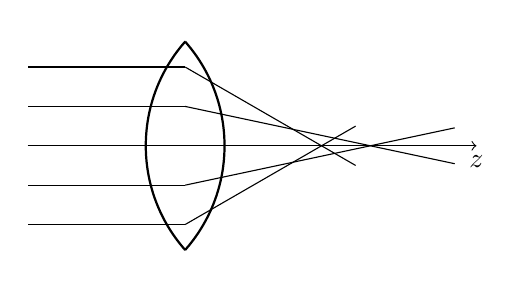
\begin{tikzpicture}


    \useasboundingbox (-1.5,-1.5) rectangle (4.3,1.5);
    %\draw (-1.5,-1.5) rectangle (4.3,1.5);
 
    \pgfmathsetmacro{\ra}{2}
    \pgfmathsetmacro{\rb}{2}
    \pgfmathsetmacro{\dr}{-3}

    \draw[->] (-1.5,0) -- (4.2,0) node[below]{$z$};    
 
     \begin{scope}
            \clip (\ra,0) circle (\ra);
            \draw[thick] (\rb + \dr,0) circle (\rb);
     \end{scope}

     \begin{scope}
        \clip (\rb + \dr,0) circle (\rb);
        \draw[thick] (\ra,0) circle (\ra);
    \end{scope}


    \draw (0.5,1) -- ++(-180:2);
    \draw (0.5,1) -- ++(-30:2.5);
    \draw (0.5,-1) -- ++(-180:2);
    \draw (0.5,-1) -- ++(+30:2.5);

    \draw (0.5,0.5) -- ++(-180:2);
    \draw (0.5,0.5) -- ++(-12:3.5);
    \draw (0.5,-0.5) -- ++(-180:2);
    \draw (0.5,-0.5) -- ++(+12:3.5);




\end{tikzpicture}



%\end{document}